\documentclass{article} % Tipo de documento

\usepackage[utf8]{inputenc} % Permite el uso de caracteres del Español

\usepackage[T1]{fontenc}

\usepackage{graphicx}

\usepackage{subfig}

% Carátula del Artículo  

\title{Reporte de Actividad 7}

\author{Brenda Leyva Amaya}

\date{24 de Marzo, 2018}
 

\begin{document}

\maketitle % Crea el título


\section{Introducción.}

En esta actividad se aborda el modelo de dos resortes acoplados con el fin de utilizar las funciones de jupyter lab para resolver las ecuaciones correspondientes y poder encontrar el comportamiento gráfico de estos resortes bajo diferentes circunstancias. Gracias a esta actividad nos acercamos a un jupyter mucho más útil para los diferentes ejercicios de modelado que se llevan a cabo en las áreas matemáticas y científicas. 

\section{Sistema de dos resortes acoplados.}

Texto de Temple H. Fay y Sarah Duncan Graham.

\vspace{0.5 cm}

En el artículo que se ha revisado se investiga el problema que aparece alejado de la discusión práctica para ser incluido únicamente como una descripción en los libros de texto. Esto es el problema de dos resortes con dos masas unidos en serie que cuelgan de un techo, en el cual se asume que las fuerzas restitutivas se comportan de acuerdo con la Ley de Hooke. Este problema se modela con un par de ecuaciones diferenciales lineales de segundo orden. 

\vspace{0.5 cm}

Se puede investigar cuando el movimiento de las dos masas está sincronizado o en fase y cuando se oponen entre sí o a 180 grados fuera de fase, esto se logra modificando las constantes de resorte. En el texto también se demuestra con ejemplos que algunos movimientos interesantes pueden surgir cuando una ligera no linealidad se introduce como un intento de incrementar las fuerzas restitutivas. 

\subsection{El modelo de resortes acoplados.}

El modelo consiste de dos resortes y dos masas. Con constantes de resorte k1 y k2 respectivamente, este se coloca a partir del techo y el peso de la masa m1 se une teniendo un resorte en su parte inferior al cual se le agrega la masa m2. Permitiendo que el sistema llegue a un punto de equilibrio, se mide el desplazamiento del centro de masa de cada una de las masas a partir del equilibrio como una función del tiempo y se denotan estas medidas como X1(t) y x2(t) respectivamente. 

\vspace{0.5 cm}

Se asume que las fuerzas restitutivas son de la forma -k1l1 y -k2l2 donde l1 y l2 son las elongaciones o compresiones de los dos resortes. Debido a que la masa superior esta unida a dos resortes, existen dos fuerzas restitutivas actuando sobre ella dadas por -k1x1 y -k2(x2-x1), mientras que la segunda masa solo siente la fuerza correspondiente a el segundo resorte. 

\subsubsection{Ejemplo 2.1.}
Se describe el movimiento de dos resortes con constantes k1=6 y k2=4 con condiciones iniciales (1,0,2,0) donde 1 y 2 son los desplazamiento y 0 y 0 son las velocidad iniciales. 

\vspace{0.5 cm}

** Resolución con jupyter lab de las ecuaciones correspondientes:

\begin{verbatim} 

# Use ODEINT to solve the differential equations defined by the vector field
from scipy.integrate import odeint
import numpy as np

# Parameter values

# Masses:
m1 = 1.0
m2 = 1.0

# Spring constants
k1 = 6.0
k2 = 4.0

# Natural lengths
L1 = 0.0
L2 = 0.0

# Friction coefficients
b1 = 0.0
b2 = 0.0

# Initial conditions
# x1 and x2 are the initial displacements; y1 and y2 are the initial velocities
x1 = 1.0
y1 = 0.0
x2 = 2.0
y2 = 0.0

# ODE solver parameters
abserr = 1.0e-8
relerr = 1.0e-6
stoptime = 50.0
numpoints = 250

# Create the time samples for the output of the ODE solver.
# I use a large number of points, only because I want to make
# a plot of the solution that looks nice.
t = [stoptime * float(i) / (numpoints - 1) for i in range(numpoints)]

# Pack up the parameters and initial conditions:
p = [m1, m2, k1, k2, L1, L2, b1, b2]
w0 = [x1, y1, x2, y2]

# Call the ODE solver.
wsol = odeint(vectorfield, w0, t, args=(p,), atol=abserr, rtol=relerr)

with open('two_springs1.dat', 'w') as f:
    # Print & save the solution.
    for t1, w1 in zip(t, wsol):
        print (t1, w1[0], w1[1], w1[2], w1[3], np.abs((np.cos(np.sqrt(2.0)*t1)-w1[0])/(np.cos(np.sqrt(2.0)*t1))), np.abs((2.0*np.cos(np.sqrt(2.0)*t1)-w1[2])/(2.0*np.cos(np.sqrt(2.0)*t1))), file=f)

\end{verbatim}

**Gráficas correspondientes al ejercicio 2.1:

\begin{verbatim} 

# Plot the solution that was generated

from numpy import loadtxt
from pylab import figure, plot, xlabel, grid, hold, legend, title, savefig
from matplotlib.font_manager import FontProperties
%matplotlib inline

t, x1, xy, x2, y2, E1, E2 = loadtxt('two_springs1.dat', unpack=True)

figure(1, figsize=(6, 4.5))

xlabel('t')
grid(True)
#hold(True)
lw = 1

plot(t, x1, 'b', linewidth=lw)
plot(t, x2, 'g', linewidth=lw)

legend((r'$x_1$', r'$x_2$'), prop=FontProperties(size=16))
title('Mass Displacements for the\nCoupled Spring-Mass System')
savefig('two_springs1-1.png', dpi=100)

\end{verbatim}



\begin{center}
 	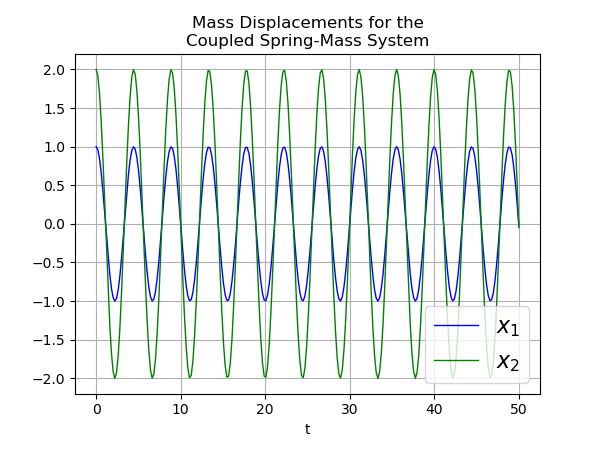
\includegraphics[width=9cm]{two_springs1-1.png}
 \end{center}





\begin{verbatim} 

%matplotlib inline

t, x1, xy, x2, y2, E1, E2 = loadtxt('two_springs1.dat', unpack=True)

figure(1, figsize=(6, 4.5))

grid(True)
lw = 1

plot(x1, x2, 'b', linewidth=lw)

legend((r'$x_1$', r'$x_2$'), prop=FontProperties(size=16))
title('x1 VS x2\nCoupled Spring-Mass System')
savefig('two_springs1-2.png', dpi=100)

\end{verbatim}


\begin{center}
 	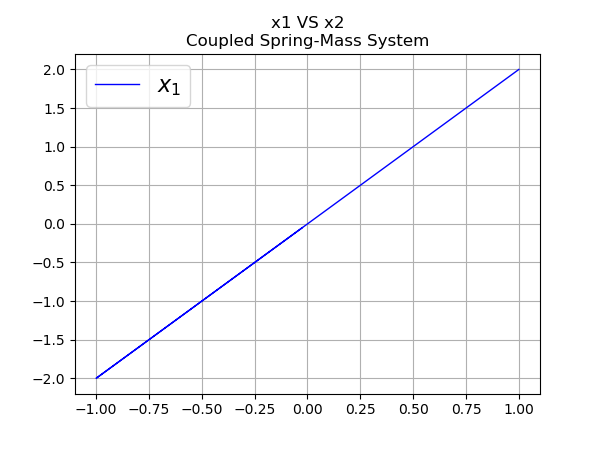
\includegraphics[width=9cm]{two_springs1-2.png}
 \end{center}


\begin{verbatim} 

%matplotlib inline

t, x1, xy, x2, y2, E1, E2 = loadtxt('two_springs1.dat', unpack=True)

figure(1, figsize=(6, 4.5))

grid(True)
lw = 1

plot(xy, x1, 'b', linewidth=lw)

plot(y2, x2, 'g', linewidth=lw)

legend((r'$x_1$', r'$x_2$'), prop=FontProperties(size=16))
title('x VS y\nCoupled Spring-Mass System')
savefig('two_springs1-3.png', dpi=100)

\end{verbatim}



\begin{center}
 	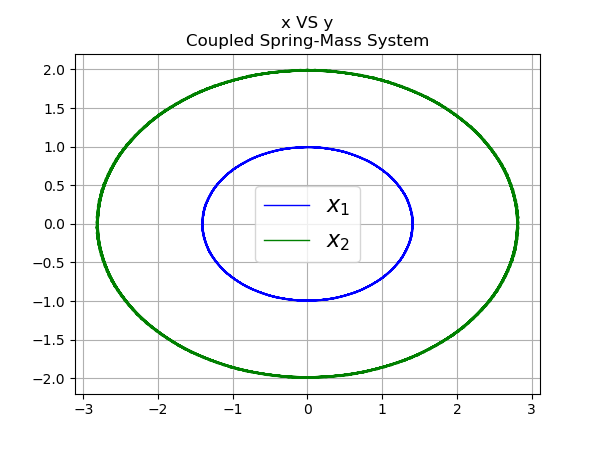
\includegraphics[width=9cm]{two_springs1-3.png}
 \end{center}



** Gráficas de error para valor calculado VS valor teórico.


\begin{verbatim} 

%matplotlib inline

t, x1, xy, x2, y2, E1, E2 = loadtxt('two_springs1.dat', unpack=True)

figure(1, figsize=(6, 4.5))

grid(True)
lw = 1

plot(t, E1, 'r', linewidth=lw)

legend((r'$x_1$', r'$x_2$'), prop=FontProperties(size=16))
title('Error 1')
savefig('two_springs1-E1.png', dpi=100)

\end{verbatim}



\begin{center}
 	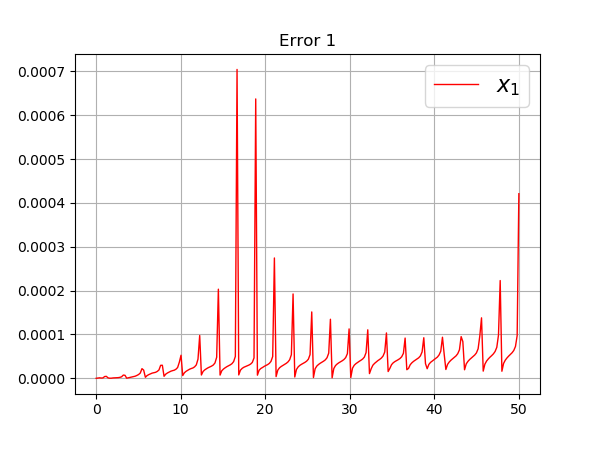
\includegraphics[width=9cm]{two_springs1-E1.png}
 \end{center}




\begin{verbatim} 

%matplotlib inline

t, x1, xy, x2, y2, E1, E2 = loadtxt('two_springs1.dat', unpack=True)

figure(1, figsize=(6, 4.5))

grid(True)
lw = 1

plot(t, E2, 'b', linewidth=lw)

legend((r'$x_1$', r'$x_2$'), prop=FontProperties(size=16))
title('Error 2')
savefig('two_springs1-E2.png', dpi=100)

\end{verbatim}



\begin{center}
 	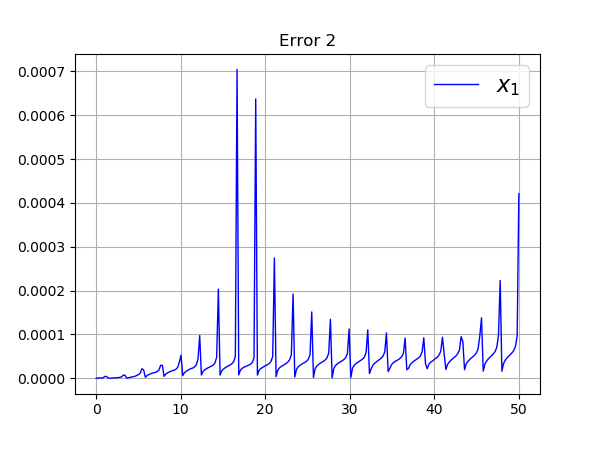
\includegraphics[width=9cm]{two_springs1-E2.png}
 \end{center}


\subsubsection{Ejemplo 2.2.}
Se describe el movimiento de dos resortes con constantes k1=6 y k2=4 con condiciones iniciales (-2,0,1,0).

\vspace{0.5 cm}

** Resolución con jupyter lab de las ecuaciones correspondientes:

\begin{verbatim} 

# Use ODEINT to solve the differential equations defined by the vector field
from scipy.integrate import odeint

# Parameter values
# Masses:
m1 = 1.0
m2 = 1.0

# Spring constants
k1 = 6.0
k2 = 4.0

# Natural lengths
L1 = 0.0
L2 = 0.0

# Friction coefficients
b1 = 0.0
b2 = 0.0

# Initial conditions
# x1 and x2 are the initial displacements; y1 and y2 are the initial velocities
x1 = -2.0
y1 = 0.0
x2 = 1.0
y2 = 0.0

# ODE solver parameters
abserr = 1.0e-8
relerr = 1.0e-6
stoptime = 25.0
numpoints = 250

# Create the time samples for the output of the ODE solver.
# I use a large number of points, only because I want to make
# a plot of the solution that looks nice.
t = [stoptime * float(i) / (numpoints - 1) for i in range(numpoints)]

# Pack up the parameters and initial conditions:
p = [m1, m2, k1, k2, L1, L2, b1, b2]
w0 = [x1, y1, x2, y2]

# Call the ODE solver.
wsol = odeint(vectorfield, w0, t, args=(p,),
              atol=abserr, rtol=relerr)

with open('two_springs2.dat', 'w') as f:
    # Print & save the solution.
    for t1, w1 in zip(t, wsol):
        print (t1, w1[0], w1[1], w1[2], w1[3], np.abs((-2.0*np.cos(2.0*np.sqrt(3.0)*t1)-w1[0])/(-2.0*np.cos(2.0*np.sqrt(3.0)*t1))), np.abs((np.cos(2.0*np.sqrt(3.0)*t1)-w1[2])/(np.cos(2.0*np.sqrt(3.0)*t1))), file=f)

\end{verbatim}

**Gráficas correspondientes al ejercicio 2.2:

\begin{verbatim} 

# Plot the solution that was generated

from numpy import loadtxt
from pylab import figure, plot, xlabel, grid, hold, legend, title, savefig
from matplotlib.font_manager import FontProperties
%matplotlib inline

t, x1, xy, x2, y2, E1, E2 = loadtxt('two_springs2.dat', unpack=True)

figure(1, figsize=(6, 4.5))

xlabel('t')
grid(True)
#hold(True)
lw = 1

plot(t, x1, 'b', linewidth=lw)
plot(t, x2, 'g', linewidth=lw)

legend((r'$x_1$', r'$x_2$'), prop=FontProperties(size=16))
title('Mass Displacements for the\nCoupled Spring-Mass System')
savefig('two_springs2-1.png', dpi=100)

\end{verbatim}



\begin{center}
 	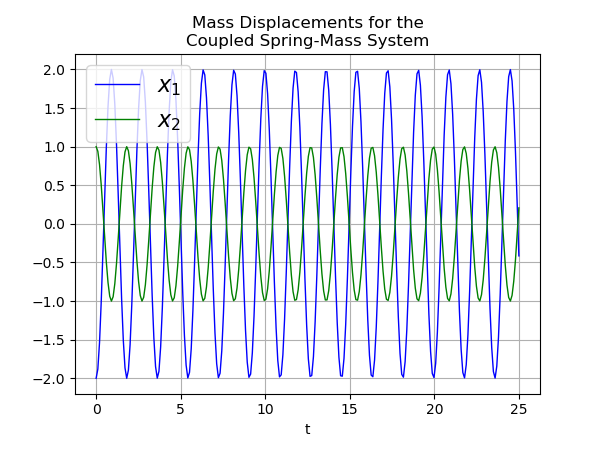
\includegraphics[width=9cm]{two_springs2-1.png}
 \end{center}





\begin{verbatim} 

%matplotlib inline

t, x1, xy, x2, y2, E1, E2 = loadtxt('two_springs2.dat', unpack=True)

figure(1, figsize=(6, 4.5))

grid(True)
lw = 1

plot(x1, x2, 'b', linewidth=lw)

legend((r'$x_1$', r'$x_2$'), prop=FontProperties(size=16))
title('x1 VS x2\nCoupled Spring-Mass System')
savefig('two_springs2-2.png', dpi=100)

\end{verbatim}


\begin{center}
 	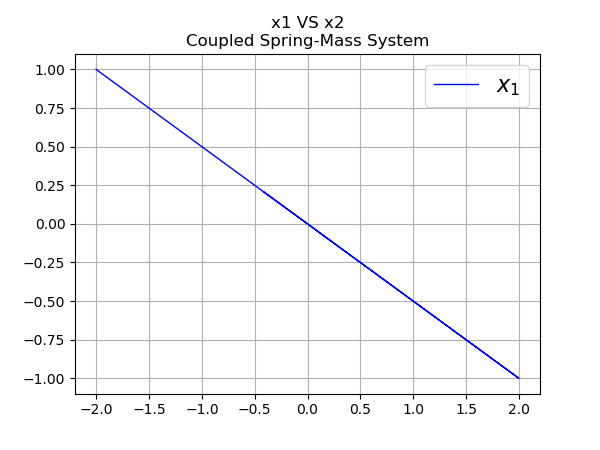
\includegraphics[width=9cm]{two_springs2-2.png}
 \end{center}


\begin{verbatim} 

%matplotlib inline

t, x1, xy, x2, y2, E1, E2 = loadtxt('two_springs2.dat', unpack=True)

figure(1, figsize=(6, 4.5))

grid(True)
lw = 1

plot(xy, x1, 'b', linewidth=lw)

plot(y2, x2, 'g', linewidth=lw)

legend((r'$x_1$', r'$x_2$'), prop=FontProperties(size=16))
title('x VS y\nCoupled Spring-Mass System')
savefig('two_springs2-3.png', dpi=100)

\end{verbatim}



\begin{center}
 	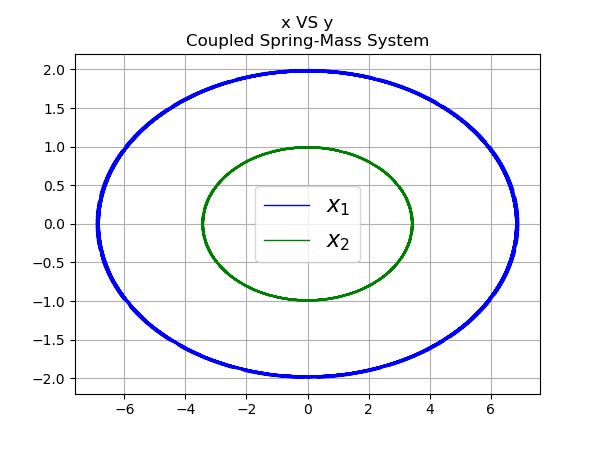
\includegraphics[width=9cm]{two_springs2-3.png}
 \end{center}



** Gráficas de error para valor calculado VS valor teórico.


\begin{verbatim} 

%matplotlib inline

t, x1, xy, x2, y2, E1, E2 = loadtxt('two_springs2.dat', unpack=True)

figure(1, figsize=(6, 4.5))

grid(True)
lw = 1

plot(t, E1, 'r', linewidth=lw)

legend((r'$x_1$', r'$x_2$'), prop=FontProperties(size=16))
title('Error 1')
savefig('two_springs2-E1.png', dpi=100)

\end{verbatim}



\begin{center}
 	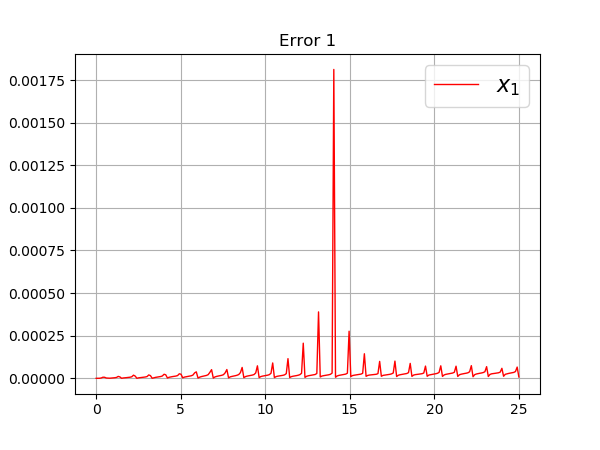
\includegraphics[width=9cm]{two_springs2-E1.png}
 \end{center}




\begin{verbatim} 

%matplotlib inline

t, x1, xy, x2, y2, E1, E2 = loadtxt('two_springs2.dat', unpack=True)

figure(1, figsize=(6, 4.5))

grid(True)
lw = 1

plot(t, E2, 'b', linewidth=lw)

legend((r'$x_1$', r'$x_2$'), prop=FontProperties(size=16))
title('Error 2')
savefig('two_springs2-E2.png', dpi=100)

\end{verbatim}



\begin{center}
 	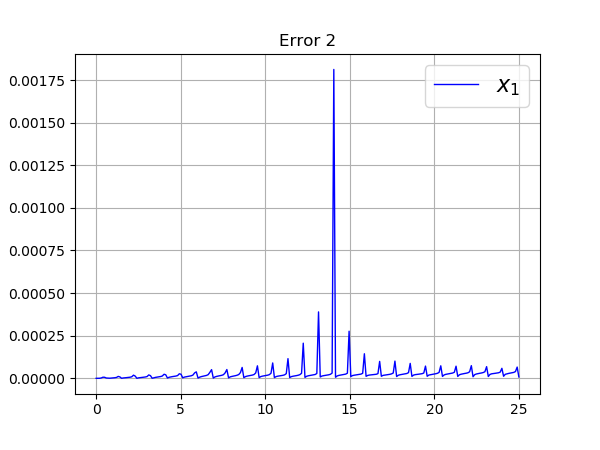
\includegraphics[width=9cm]{two_springs2-E2.png}
 \end{center}




\subsubsection{Ejemplo 2.3.}
Se describe el movimiento de dos resortes con constantes k1=0.4 y k2=1.808 con condiciones iniciales (1/2,0,-1/2,7/10).

\vspace{0.5 cm}

** Resolución con jupyter lab de las ecuaciones correspondientes:

\begin{verbatim} 

def vectorfield(w, t, p):
    """
    Defines the differential equations for the coupled spring-mass system.

    Arguments:
        w :  vector of the state variables:
                  w = [x1,y1,x2,y2]
        t :  time
        p :  vector of the parameters:
                  p = [m1,m2,k1,k2,L1,L2,b1,b2]
    """
    x1, y1, x2, y2 = w
    m1, m2, k1, k2, L1, L2, b1, b2 = p

    # Create f = (x1',y1',x2',y2'):
    f = [y1,(-b1 * y1 - k1 * (x1 - L1) + k2 * (x2 - x1 - L2)) / m1,y2,(-b2 * y2 - k2 * (x2 - x1 - L2)) / m2]
    return f


# Use ODEINT to solve the differential equations defined by the vector field
from scipy.integrate import odeint

# Parameter values
# Masses:
m1 = 1.0
m2 = 1.0

# Spring constants
k1 = 0.4
k2 = 1.808

# Natural lengths
L1 = 0.0
L2 = 0.0

# Friction coefficients
b1 = 0.0
b2 = 0.0

# Initial conditions
# x1 and x2 are the initial displacements; y1 and y2 are the initial velocities
x1 = 0.5
y1 = 0.0
x2 = -0.5
y2 = 7/10

# ODE solver parameters
abserr = 1.0e-8
relerr = 1.0e-6
stoptime = 50.0
numpoints = 250

# Create the time samples for the output of the ODE solver.
# I use a large number of points, only because I want to make
# a plot of the solution that looks nice.
t = [stoptime * float(i) / (numpoints - 1) for i in range(numpoints)]

# Pack up the parameters and initial conditions:
p = [m1, m2, k1, k2, L1, L2, b1, b2]
w0 = [x1, y1, x2, y2]

# Call the ODE solver.
wsol = odeint(vectorfield, w0, t, args=(p,), atol=abserr, rtol=relerr)

with open('two_springs3.dat', 'w') as f:
    # Print & save the solution.
    for t1, w1 in zip(t, wsol):
        print (t1, w1[0], w1[1], w1[2], w1[3], file=f)

\end{verbatim}


**Gráficas correspondientes al ejercicio 2.3:

\begin{verbatim} 

# Plot the solution that was generated

from numpy import loadtxt
from pylab import figure, plot, xlabel, grid, hold, legend, title, savefig
from matplotlib.font_manager import FontProperties
%matplotlib inline

t, x1, xy, x2, y2 = loadtxt('two_springs3.dat', unpack=True)

figure(1, figsize=(6, 4.5))

xlabel('t')
grid(True)
#hold(True)
lw = 1

plot(t, x1, 'b', linewidth=lw)
plot(t, x2, 'g', linewidth=lw)

legend((r'$x_1$', r'$x_2$'), prop=FontProperties(size=16))
title('Mass Displacements for the\nCoupled Spring-Mass System')
savefig('two_springs3-1.png', dpi=100)

\end{verbatim}



\begin{center}
 	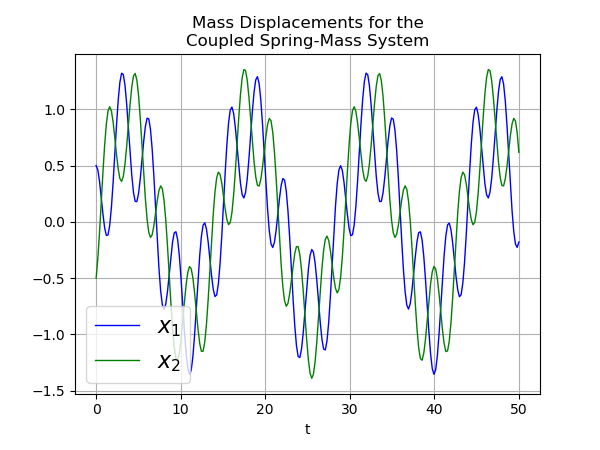
\includegraphics[width=9cm]{two_springs3-1.png}
 \end{center}



\begin{verbatim} 

%matplotlib inline

t, x1, xy, x2, y2 = loadtxt('two_springs3.dat', unpack=True)

figure(1, figsize=(6, 4.5))

grid(True)
lw = 1

plot(x1, x2, 'b', linewidth=lw)

legend((r'$x_1$', r'$x_2$'), prop=FontProperties(size=16))
title('x1 VS x2\nCoupled Spring-Mass System')
savefig('two_springs3-2.png', dpi=100)

\end{verbatim}


\begin{center}
 	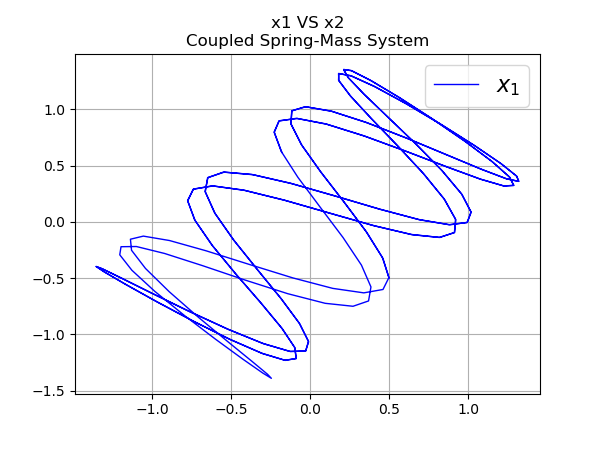
\includegraphics[width=9cm]{two_springs3-2.png}
 \end{center}


\begin{verbatim} 

%matplotlib inline

t, x1, xy, x2, y2 = loadtxt('two_springs3.dat', unpack=True)

figure(1, figsize=(6, 4.5))

grid(True)
lw = 1

plot(x1, xy, 'b', linewidth=lw)

legend((r'$x_1$', r'$x_2$'), prop=FontProperties(size=16))
title('x VS y\nCoupled Spring-Mass System')
savefig('two_springs3-3.png', dpi=100)

\end{verbatim}



\begin{center}
 	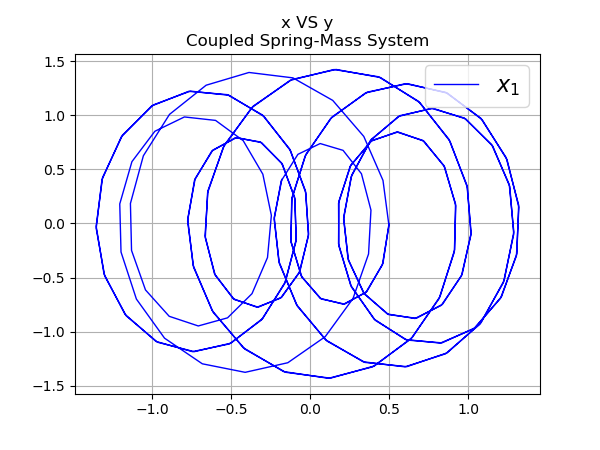
\includegraphics[width=9cm]{two_springs3-3.png}
 \end{center}



\begin{verbatim} 

%%matplotlib inline

t, x1, xy, x2, y2 = loadtxt('two_springs3.dat', unpack=True)

figure(1, figsize=(6, 4.5))

grid(True)
lw = 1

plot(x2, y2, 'g', linewidth=lw)

legend((r'$x_1$', r'$x_2$'), prop=FontProperties(size=16))
title('x VS y\nCoupled Spring-Mass System')
savefig('two_springs3-4.png', dpi=100)

\end{verbatim}



\begin{center}
 	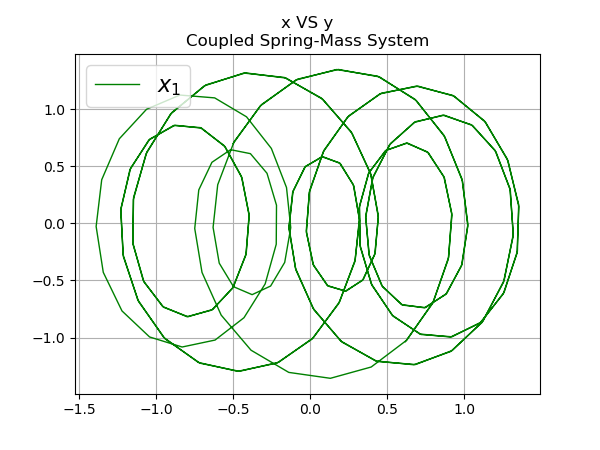
\includegraphics[width=9cm]{two_springs3-4.png}
 \end{center}


\subsubsection{Ejemplo 2.4.}
Se describe el movimiento de dos resortes con constantes k1=0.4 y k2=1.808 con condiciones iniciales (1,1/2,2,1/2) y coeficientes de fricción b1=0.1 y b2=0.2.

\vspace{0.5 cm}

** Resolución con jupyter lab de las ecuaciones correspondientes:

\begin{verbatim} 

def vectorfield(w, t, p):
    """
    Defines the differential equations for the coupled spring-mass system.

    Arguments:
        w :  vector of the state variables:
                  w = [x1,y1,x2,y2]
        t :  time
        p :  vector of the parameters:
                  p = [m1,m2,k1,k2,L1,L2,b1,b2]
    """
    x1, y1, x2, y2 = w
    m1, m2, k1, k2, L1, L2, b1, b2 = p

    # Create f = (x1',y1',x2',y2'):
    f = [y1,(-b1 * y1 - k1 * (x1 - L1) + k2 * (x2 - x1 - L2)) / m1,y2,(-b2 * y2 - k2 * (x2 - x1 - L2)) / m2]
    return f

# Use ODEINT to solve the differential equations defined by the vector field
from scipy.integrate import odeint

# Parameter values
# Masses:
m1 = 1.0
m2 = 1.0

# Spring constants
k1 = 0.4
k2 = 1.808

# Natural lengths
L1 = 0.0
L2 = 0.0

# Friction coefficients
b1 = 0.1
b2 = 0.2

# Initial conditions
# x1 and x2 are the initial displacements; y1 and y2 are the initial velocities
x1 = 1.0
y1 = 0.5
x2 = 2.0
y2 = 0.5

# ODE solver parameters
abserr = 1.0e-8
relerr = 1.0e-6
stoptime = 50.0
numpoints = 250

# Create the time samples for the output of the ODE solver.
# I use a large number of points, only because I want to make
# a plot of the solution that looks nice.
t = [stoptime * float(i) / (numpoints - 1) for i in range(numpoints)]

# Pack up the parameters and initial conditions:
p = [m1, m2, k1, k2, L1, L2, b1, b2]
w0 = [x1, y1, x2, y2]

# Call the ODE solver.
wsol = odeint(vectorfield, w0, t, args=(p,), atol=abserr, rtol=relerr)

with open('two_springs4.dat', 'w') as f:
    # Print & save the solution.
    for t1, w1 in zip(t, wsol):
        print (t1, w1[0], w1[1], w1[2], w1[3], file=f) 

\end{verbatim}


**Gráficas correspondientes al ejercicio 2.4:

\begin{verbatim} 

# Plot the solution that was generated

from numpy import loadtxt
from pylab import figure, plot, xlabel, grid, hold, legend, title, savefig
from matplotlib.font_manager import FontProperties
%matplotlib inline

t, x1, xy, x2, y2 = loadtxt('two_springs4.dat', unpack=True)

figure(1, figsize=(6, 4.5))

xlabel('t')
grid(True)
#hold(True)
lw = 1

plot(t, x1, 'b', linewidth=lw)
plot(t, x2, 'g', linewidth=lw)

legend((r'$x_1$', r'$x_2$'), prop=FontProperties(size=16))
title('Mass Displacements for the\nCoupled Spring-Mass System')
savefig('two_springs4-1.png', dpi=100)

\end{verbatim}



\begin{center}
 	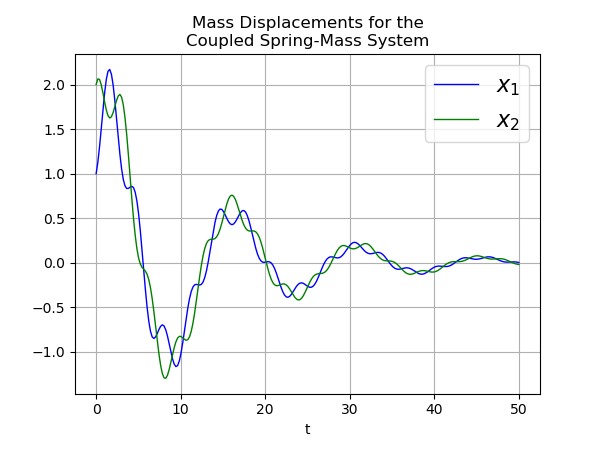
\includegraphics[width=9cm]{two_springs4-1.png}
 \end{center}



\begin{verbatim} 

%matplotlib inline

t, x1, xy, x2, y2 = loadtxt('two_springs4.dat', unpack=True)

figure(1, figsize=(6, 4.5))

grid(True)
lw = 1

plot(x1, x2, 'b', linewidth=lw)

legend((r'$x_1$', r'$x_2$'), prop=FontProperties(size=16))
title('x1 VS x2\nCoupled Spring-Mass System')
savefig('two_springs4-2.png', dpi=100)

\end{verbatim}


\begin{center}
 	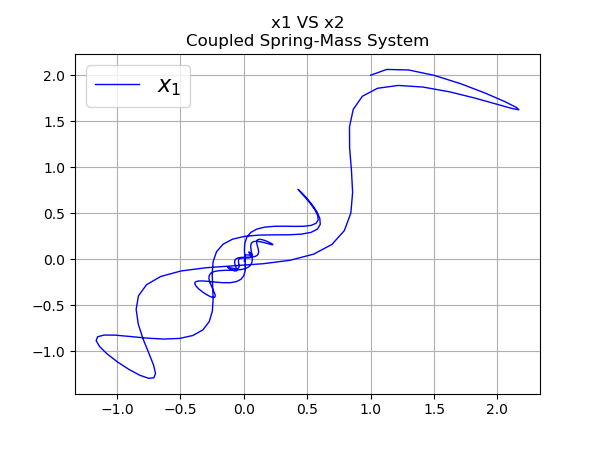
\includegraphics[width=9cm]{two_springs4-2.png}
 \end{center}


\begin{verbatim} 

%matplotlib inline

t, x1, xy, x2, y2 = loadtxt('two_springs4.dat', unpack=True)

figure(1, figsize=(6, 4.5))

grid(True)
lw = 1

plot(x1, xy, 'b', linewidth=lw)

legend((r'$x_1$', r'$x_2$'), prop=FontProperties(size=16))
title('x VS y\nCoupled Spring-Mass System')
savefig('two_springs4-3.png', dpi=100)

\end{verbatim}



\begin{center}
 	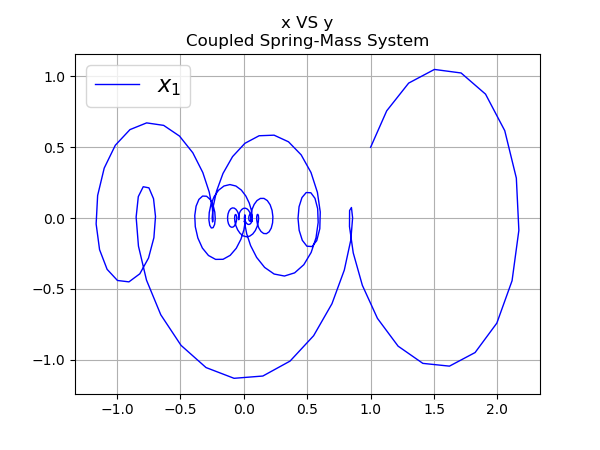
\includegraphics[width=9cm]{two_springs4-3.png}
 \end{center}



\begin{verbatim} 

%%matplotlib inline

t, x1, xy, x2, y2 = loadtxt('two_springs4.dat', unpack=True)

figure(1, figsize=(6, 4.5))

grid(True)
lw = 1

plot(x2, y2, 'g', linewidth=lw)

legend((r'$x_1$', r'$x_2$'), prop=FontProperties(size=16))
title('x VS y\nCoupled Spring-Mass System')
savefig('two_springs4-4.png', dpi=100)

\end{verbatim}



\begin{center}
 	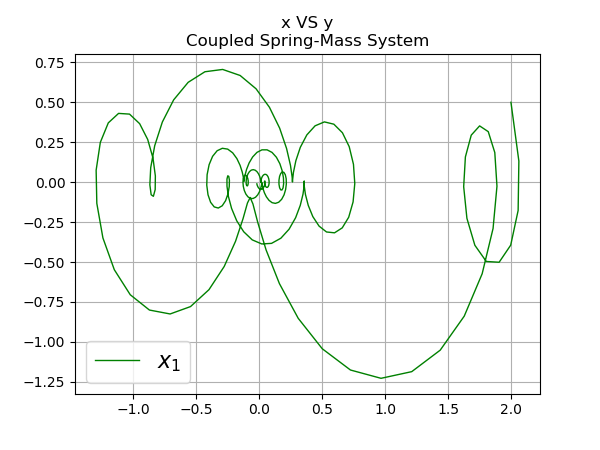
\includegraphics[width=9cm]{two_springs4-4.png}
 \end{center}


\subsection{Agregando no linealidad.}

Si se asume que las fuerzas restitutivas no son lineales, lo cual es muy probable para vibraciones de larga duración, se puede modificar el modelo para ajustarlo a estas condiciones. Se supone entonces que la fuerza restitutiva tiene la forma -kx+$\mu x^3$.

\vspace{0.5 cm}

El rango de movimientos para un modelo no linear es mucho más complejo que el del lineal. Para observar el fenómeno se desarrollan lo siguientes ejemplos:


\subsubsection{Ejemplo 3.1}

Se toman dos masas m1=m2=1. Describimos el movimiento para resorte con constantes k1=0.4 y k2=1.808, coeficientes de amortiguamiento b1=0 y b2=0, coeficientes no lineales $\mu$1=-1/6 y $\mu$2=-1/10 con condiciones iniciales (1,0,-1/2,0).

\vspace{0.5 cm}

** Resolución de las ecuaciones para ejemplo 3.1:

\begin{verbatim} 

from scipy.integrate import odeint

# Parameter values
# Masses:
m1 = 1.0
m2 = 1.0

# Spring constants
k1 = 0.4
k2 = 1.808

# Friction coefficients
b1 = 0.0
b2 = 0.0


#Coeficientes no lineales
n1=-1/6
n2=-1/10

# Initial conditions
# x1 and x2 are the initial displacements; y1 and y2 are the initial velocities
x1 = 1.0
y1 = 0.0
x2 = -1/2
y2 = 0.0

# ODE solver parameters
abserr = 1.0e-8
relerr = 1.0e-6
stoptime = 50.0
numpoints = 250

# Create the time samples for the output of the ODE solver.
# I use a large number of points, only because I want to make
# a plot of the solution that looks nice.
t = [stoptime * float(i) / (numpoints - 1) for i in range(numpoints)]

# Pack up the parameters and initial conditions:
p = [m1, m2, k1, k2, b1, b2, n1, n2]
w0 = [x1, y1, x2, y2]

# Call the ODE solver.
wsol = odeint(vectorfield, w0, t, args=(p,),
              atol=abserr, rtol=relerr)

with open('nonlinear3.1.dat', 'w') as f:
    # Print & save the solution.
    for t1, w1 in zip(t, wsol):
        print (t1, w1[0], w1[1], w1[2], w1[3], file=f)

\end{verbatim}


** Imágenes correspondientes al ejemplo 3.1:


\begin{verbatim} 

import numpy
from numpy import loadtxt
from pylab import figure, plot, xlabel, grid, hold, legend, title, savefig, ylabel
from matplotlib.font_manager import FontProperties
import matplotlib.pyplot as plt
%matplotlib inline

t, x1, y1, x2, y2 = loadtxt('nonlinear3.1.dat', unpack=True)

figure(1, figsize=(6, 4.5))

xlabel('x')
ylabel('y')
grid(True)
lw = 1.5

plot(x1, y1, 'y', linewidth=lw)
plt.xlim=[-2,2]
plt.ylim=[-2,2]

title('Phase plot for x1')
savefig('nonlinear3.1.1.png', dpi=100)

\end{verbatim}


\begin{center}
	\includegraphics[width=9cm]{nonlinear3_1_1.png}
\end{center}


\begin{verbatim} 

import numpy
from numpy import loadtxt
from pylab import figure, plot, xlabel, grid, hold, legend, title, savefig, ylabel
from matplotlib.font_manager import FontProperties
import matplotlib.pyplot as plt
%matplotlib inline

t, x1, y1, x2, y2 = loadtxt('nonlinear3.1.dat', unpack=True)

figure(1, figsize=(6, 4.5))

xlabel('x')
ylabel('y')
grid(True)
lw = 1.5

plot(x2, y2, 'b', linewidth=lw)
plt.xlim=[-2,2]
plt.ylim=[-2,2]

title('Phase plot for x1')
savefig('nonlinear3.1.2.png', dpi=100)

\end{verbatim}


\begin{center}
	\includegraphics[width=9cm]{nonlinear3_1_2.png}
\end{center}



\begin{verbatim} 

import numpy
from numpy import loadtxt
from pylab import figure, plot, xlabel, grid, hold, legend, title, savefig, ylabel
from matplotlib.font_manager import FontProperties
import matplotlib.pyplot as plt
%matplotlib inline

t, x1, y1, x2, y2 = loadtxt('nonlinear3.1.dat', unpack=True)

figure(1, figsize=(6, 4.5))

xlabel('t')
ylabel('x')
grid(True)
lw = 1.5

plot(t, x1, 'g', linewidth=lw)

title('Phase plot for x1')
savefig('nonlinear3.1.3.png', dpi=100)

\end{verbatim}


\begin{center}
	\includegraphics[width=9cm]{nonlinear3_1_3.png}
\end{center}



\begin{verbatim} 

import numpy
from numpy import loadtxt
from pylab import figure, plot, xlabel, grid, hold, legend, title, savefig, ylabel
from matplotlib.font_manager import FontProperties
import matplotlib.pyplot as plt
%matplotlib inline

t, x1, y1, x2, y2 = loadtxt('nonlinear3.1.dat', unpack=True)

figure(1, figsize=(6, 4.5))

xlabel('t')
ylabel('x')
grid(True)
lw = 1.5

plot(t, x2, 'b', linewidth=lw)

title('Phase plot for x1')
savefig('nonlinear3.1.4.png', dpi=100)

\end{verbatim}


\begin{center}
	\includegraphics[width=9cm]{nonlinear3_1_4.png}
\end{center}




\begin{verbatim} 

import numpy
from numpy import loadtxt
from pylab import figure, plot, xlabel, grid, hold, legend, title, savefig, ylabel
from matplotlib.font_manager import FontProperties
import matplotlib.pyplot as plt
%matplotlib inline

t, x1, y1, x2, y2 = loadtxt('nonlinear3.1.dat', unpack=True)

figure(1, figsize=(6, 4.5))

xlabel('t')
ylabel('x')
grid(True)
lw = 1.5

plot(t, x1, 'orange', linewidth=lw)
plot(t, x2, 'blue', linewidth=lw)

title('Phase plot for x1')
savefig('nonlinear3.1.5.png', dpi=100)

\end{verbatim}


\begin{center}
	\includegraphics[width=9cm]{nonlinear3_1_5.png}
\end{center}




\begin{verbatim} 

import numpy
from numpy import loadtxt
from pylab import figure, plot, xlabel, grid, hold, legend, title, savefig, ylabel
from matplotlib.font_manager import FontProperties
import matplotlib.pyplot as plt
%matplotlib inline

t, x1, y1, x2, y2 = loadtxt('nonlinear3.1.dat', unpack=True)

figure(1, figsize=(6, 4.5))

xlabel('x1')
ylabel('x2')
grid(True)
lw = 1.5

plot(x1, x2, 'orange', linewidth=lw)

title('Phase plot for x1')
savefig('nonlinear3.1.6.png', dpi=100)

\end{verbatim}


\begin{center}
	\includegraphics[width=9cm]{nonlinear3_1_6.png}
\end{center}


\subsubsection{Ejemplo 3.2}

Se toman dos masas m1=m2=1. Describimos el movimiento para resorte con constantes k1=0.4 y k2=1.808, coeficientes de amortiguamiento b1=0 y b2=0, coeficientes no lineales $\mu$1=-1/6 y $\mu$2=-1/10 con condiciones iniciales (-0.5,1/2,3.001,5.9).

\vspace{0.5 cm}

** Resolución de las ecuaciones para ejemplo 3.2:


\begin{verbatim} 

from scipy.integrate import odeint

# Valor de los parametros
# Masas:
m1 = 1.0
m2 = 1.0
# Constante del resorte
k1 = 0.4
k2 = 1.808
# Longitudes naturales
L1 = 0.0
L2 = 0.0
# Coeficientes de fricción
b1 = 0.0
b2 = 0.0
# Coeficiente de no linealidad
n1 = -(1.0/6.0)
n2 = -(1.0/10.0)

# Condiciones iniciales
# x1 and x2 son las pocisiones iniciales(contando la longitud de L), y y1 y y2 son las velocidades
x1 = -0.5
y1 = 0.5
x2 = 3.001
y2 = 5.9

# Parametros de la ED
abserr = 1.0e-8
relerr = 1.0e-6
stoptime = 200.0
numpoints = 2150

# Create the time samples for the output of the ODE solver.
# I use a large number of points, only because I want to make
# a plot of the solution that looks nice.
t = [stoptime * float(i) / (numpoints - 1) for i in range(numpoints)]

# Pack up the parameters and initial conditions:
p = [m1, m2, k1, k2, L1, L2, b1, b2, n1, n2]
w0 = [x1, y1, x2, y2]

# Call the ODE solver.
wsol = odeint(vectorfield, w0, t, args=(p,),
              atol=abserr, rtol=relerr)

with open('nonlinear3.2.dat', 'w') as f:
    # Print & save the solution.
    for t1, w1 in zip(t, wsol):
        print (t1, w1[0], w1[1], w1[2], w1[3],file=f)



\end{verbatim}


** Imágenes correspondientes al ejemplo 3.2:


\begin{verbatim} 

import numpy 
from numpy import loadtxt
from pylab import figure, plot, xlabel, grid, hold, legend, title, savefig, ylabel
from matplotlib.font_manager import FontProperties
import matplotlib.pyplot as plt
%matplotlib inline

t, x1, y1, x2, y2 = loadtxt('nonlinear3.2.dat', unpack=True)

figure(1, figsize=(6, 4.5))

xlabel('x')
ylabel('v')
grid(True)
lw = 1.5

plot(x1, y1, 'limegreen', linewidth=lw)

plt.axhline(0, color='black',linewidth=0.5)
plt.axvline(0, color='black',linewidth=0.5)

plt.xlim(-10,10)
plt.ylim(-10,10)

title('Phase plot for x1')
savefig('nonlinear3.2.1.png', dpi=100)


\end{verbatim}


\begin{center}
	\includegraphics[width=9cm]{nonlinear3_2_1.png}
\end{center}


\begin{verbatim} 
figure(1, figsize=(6, 4.5))

xlabel('x')
ylabel('v')
grid(True)
lw = 1.5

plot(x2, y2, "orange", linewidth=lw)
plt.axhline(0, color='black',linewidth=0.5)
plt.axvline(0, color='black',linewidth=0.5)

plt.xlim(-10,10)
plt.ylim(-10,10)

title('Phase plot for x2')
savefig('nonlinear3.2.2.png', dpi=100)

\end{verbatim}


\begin{center}
	\includegraphics[width=9cm]{nonlinear3_2_2.png}
\end{center}



\begin{verbatim} 

figure(1, figsize=(6, 4.5))

grid(True)
lw = 1.5

plot(x1, x2, 'purple', linewidth=lw)
plt.axhline(0, color='black',linewidth=0.5)
plt.axvline(0, color='black',linewidth=0.5)
plt.xlim(-10,10)
plt.ylim(-10,10)

title('x1 vs x2')
savefig('nonlinear3.2.3.png', dpi=100)

\end{verbatim}


\begin{center}
	\includegraphics[width=9cm]{nonlinear3_2_3.png}
\end{center}



\subsubsection{Ejemplo 3.3}

Se toman dos masas m1=m2=1. Describimos el movimiento para resorte con constantes k1=0.4 y k2=1.808, coeficientes de amortiguamiento b1=0 y b2=0, coeficientes no lineales $\mu$1=-1/6 y $\mu$2=-1/10 con condiciones iniciales (-0.6,1/2,3.001,5.9).

\vspace{0.5 cm}

** Resolución de las ecuaciones para ejemplo 3.3:

\begin{verbatim} 

# Masas:
m1 = 1.0
m2 = 1.0
# Constante del resorte
k1 = 0.4
k2 = 1.808
# Longitudes naturales
L1 = 0.0
L2 = 0.0
# Coeficientes de fricción
b1 = 0.0
b2 = 0.0
# Coeficiente de no linealidad
n1 = -(1.0/6.0)
n2 = -(1.0/10.0)

# Condiciones iniciales
# x1 and x2 son las pocisiones iniciales(contando la longitud de L), y y1 y y2 son las velocidades
x1 = -0.6
y1 = 0.5
x2 = 3.001
y2 = 5.9

# Parametros de la ED
abserr = 1.0e-8
relerr = 1.0e-6
stoptime = 200.0
numpoints = 2150

# Create the time samples for the output of the ODE solver.
# I use a large number of points, only because I want to make
# a plot of the solution that looks nice.
t = [stoptime * float(i) / (numpoints - 1) for i in range(numpoints)]

# Pack up the parameters and initial conditions:
p = [m1, m2, k1, k2, L1, L2, b1, b2, n1, n2]
w0 = [x1, y1, x2, y2]

# Call the ODE solver.
wsol = odeint(vectorfield, w0, t, args=(p,),
              atol=abserr, rtol=relerr)

with open('nonlinear3.3.dat', 'w') as f:
    # Print & save the solution.
    for t1, w1 in zip(t, wsol):
        print (t1, w1[0], w1[1], w1[2], w1[3],file=f)

\end{verbatim}


** Imágenes correspondientes al ejemplo 3.3:


\begin{verbatim} 

import numpy 
from numpy import loadtxt
from pylab import figure, plot, xlabel, grid, hold, legend, title, savefig, ylabel
from matplotlib.font_manager import FontProperties
import matplotlib.pyplot as plt
%matplotlib inline

t, x1, y1, x2, y2 = loadtxt('nonlinear3.3.dat', unpack=True)

figure(1, figsize=(6, 4.5))

xlabel('x')
ylabel('v')
grid(True)
lw = 1.5

plot(x1, y1, 'green', linewidth=lw)

plt.axhline(0, color='black',linewidth=0.5)
plt.axvline(0, color='black',linewidth=0.5)

plt.xlim(-10,10)
plt.ylim(-10,10)

title('Phase plot for x1')
savefig('nonlinear3.3.1.png', dpi=100)


\end{verbatim}


\begin{center}
	\includegraphics[width=9cm]{nonlinear3_3_1.png}
\end{center}


\begin{verbatim} 

figure(1, figsize=(6, 4.5))

xlabel('x')
ylabel('v')
grid(True)
lw = 1.5

plot(x2, y2, "red", linewidth=lw)
plt.axhline(0, color='black',linewidth=0.5)
plt.axvline(0, color='black',linewidth=0.5)

plt.xlim(-10,10)
plt.ylim(-10,10)

title('Phase plot for x2')
savefig('nonlinear3.3.2.png', dpi=100)

\end{verbatim}


\begin{center}
	\includegraphics[width=9cm]{nonlinear3_3_2.png}
\end{center}


\begin{verbatim} 

figure(1, figsize=(6, 4.5))

grid(True)
lw = 1.5

plot(x1, x2, 'limegreen', linewidth=lw)
plt.axhline(0, color='black',linewidth=0.5)
plt.axvline(0, color='black',linewidth=0.5)
plt.xlim(-10,10)
plt.ylim(-10,10)

title('x1 vs x2')
savefig('nonlinear3.3.3.png', dpi=100)

\end{verbatim}


\begin{center}
	\includegraphics[width=9cm]{nonlinear3_3_3.png}
\end{center}


\subsection{Fuerza adicional.}

ES un concepto sencillo el de agregar una fuerza adicional al sistema, así cada peso puede tener un movimiento diferente. El rango de movimientos para sistemas no lineales con una fuerza adicional es muy extenso, sin embargo las soluciones a estos sistemas pueden volverse muy complejas, aquí se presentan ejemplos sencillos de lo que puede ocurrir en este escenario. 

\subsubsection{Ejemplo 4.1}

Se toman dos masas m1=m2=1. Describimos el movimiento para resorte con constantes k1=2/5 y k2=1.808, coeficientes de amortiguamiento b1=1/10 y b2=1/5, coeficientes no lineales $\mu$1=1/6 y $\mu$2=1/10, amplitudes forzadas de F1=1/3 y F2=1/5, con frecuencias de forzado $\omega$1=1 y $\omega$2=3/5 con condiciones iniciales (0.7,0,0.1,0).

\vspace{0.5 cm}

** Resolución de las ecuaciones para ejemplo 4.1:


\begin{verbatim} 

from scipy.integrate import odeint

# Masas:
m1 = 1.0
m2 = 1.0
# Constante del resorte
k1 = (2.0/5.0)
k2 = 1
# Longitudes naturales
L1 = 0.0
L2 = 0.0
# Coeficientes de fricción
b1 = (1.0/10.0)
b2 = (1.0/5.0)
# Coeficiente de no linealidad
n1 = (1.0/6.0)
n2 = (1.0/10.0)
#Amplitud
F1 = (1.0/3.0)
F2 = (1.0/5.0)
#Frecuencia
w1 = 1
w2 = (3.0/5.0)

# Condiciones iniciales
# x1 and x2 son las pocisiones iniciales(contando la longitud de L), y y1 y y2 son las velocidades
x1 = 0.7
y1 = 0
x2 = 0.1
y2 = 0

# Parametros de la ED
abserr = 1.0e-8
relerr = 1.0e-6
stoptime = 250.0
numpoints = 2150

# Create the time samples for the output of the ODE solver.
# I use a large number of points, only because I want to make
# a plot of the solution that looks nice.
t = [stoptime * float(i) / (numpoints - 1) for i in range(numpoints)]

# Pack up the parameters and initial conditions:
p = [m1, m2, k1, k2, L1, L2, b1, b2, n1, n2, F1, F2, w1, w2]
w0 = [x1, y1, x2, y2]

# Call the ODE solver.
wsol = odeint(vectorfield, w0, t, args=(p,),
              atol=abserr, rtol=relerr)

with open('addedforce4.1.dat', 'w') as f:
    # Print & save the solution.
    for t1, w1 in zip(t, wsol):
        print (t1, w1[0], w1[1], w1[2], w1[3],file=f)


\end{verbatim}


** Imágenes correspondientes al ejemplo 4.1:


\begin{verbatim} 

import numpy 
from numpy import loadtxt
from pylab import figure, plot, xlabel, grid, hold, legend, title, savefig, ylabel
from matplotlib.font_manager import FontProperties
import matplotlib.pyplot as plt
%matplotlib inline

t, x1, y1, x2, y2 = loadtxt('addedforce4.1.dat', unpack=True)

figure(1, figsize=(6, 4.5))

xlabel('x')
ylabel('v')
grid(True)
lw = 1.5

plot(x1, y1, 'teal', linewidth=lw)

plt.axhline(0, color='black',linewidth=0.5)
plt.axvline(0, color='black',linewidth=0.5)

plt.xlim(-1,1)
plt.ylim(-1,1)

title('Phase plot for x1')
savefig('addedforce4.1.1.png', dpi=100)


\end{verbatim}


\begin{center}
	\includegraphics[width=9cm]{addedforce4_1_1.png}
\end{center}


\begin{verbatim} 

figure(1, figsize=(6, 4.5))

xlabel('x')
ylabel('v')
grid(True)
lw = 1.5

plot(x2, y2, "blue", linewidth=lw)
plt.axhline(0, color='black',linewidth=0.5)
plt.axvline(0, color='black',linewidth=0.5)

plt.xlim(-1.5,1.5)
plt.ylim(-1.5,1.5)

title('Phase plot for x2')
savefig('addedforce4.1.2.png', dpi=100)


\end{verbatim}


\begin{center}
	\includegraphics[width=9cm]{addedforce4_1_2.png}
\end{center}



\begin{verbatim} 

figure(1, figsize=(6, 4.5))

xlabel('t')
ylabel('x')
grid(True)
lw = 1.5

plot(t, x1, 'orange', linewidth=lw)
plt.axhline(0, color='black',linewidth=0.5)
plt.axvline(0, color='black',linewidth=0.5)

plt.xlim(0,150)
plt.ylim(-2,2)

title('x1')
savefig('addedforce4.1.3.png', dpi=100)


\end{verbatim}


\begin{center}
	\includegraphics[width=9cm]{addedforce4_1_3.png}
\end{center}



\begin{verbatim} 

figure(1, figsize=(6, 4.5))

xlabel('t')
ylabel('x')
grid(True)
lw = 1.5

plot(t, x2, 'violet', linewidth=lw)
plt.axhline(0, color='black',linewidth=0.5)
plt.axvline(0, color='black',linewidth=0.5)

plt.xlim(0,150)
plt.ylim(-2,2)

title('x2')
savefig('addedforce4.1.4.png', dpi=100)

\end{verbatim}


\begin{center}
	\includegraphics[width=9cm]{addedforce4_1_4.png}
\end{center}


\begin{verbatim} 

t, x1, y1, x2, y2 = loadtxt('addedforce4.1.dat', unpack=True)

figure(1, figsize=(6, 4.5))

xlabel('t')
ylabel('x')
grid(True)
lw = 1.5

plot(t, x1, 'blue', linewidth=lw)
plot(t, x2, 'turquoise', linewidth=lw)
plt.axhline(0, color='black',linewidth=0.5)
plt.axvline(0, color='black',linewidth=0.5)

y = [-2, -1.5, -1,-0.5,0,0.5,1,1.5,2]
plt.yticks(y)

legend((r'$x_1$', r'$x_2$'), prop=FontProperties(size=16))
title('Posición de las Masas para')
savefig('addedforce4.1.5.png', dpi=100)

\end{verbatim}


\begin{center}
	\includegraphics[width=9cm]{addedforce4_1_5.png}
\end{center}


\begin{verbatim} 

t, x1, y1, x2, y2 = loadtxt('addedforce4.1.dat', unpack=True, skiprows=1828)

figure(1, figsize=(6, 4.5))

grid(True)
lw = 1.5

plot(x1, x2, 'red', linewidth=lw)
plt.axhline(0, color='black',linewidth=0.5)
plt.axvline(0, color='black',linewidth=0.5)

plt.xlim(-1,1)
plt.ylim(-1,1)

title('x1 vs x2')
savefig('addedforce4.1.6.png', dpi=100)


\end{verbatim}


\begin{center}
	\includegraphics[width=9cm]{addedforce4_1_6.png}
\end{center}


** Resolución de ejemplo 4.1 parte 2:


\begin{verbatim} 

from scipy.integrate import odeint

# Masas:
m1 = 1.0
m2 = 1.0
# Constante del resorte
k1 = (2.0/5.0)
k2 = 1
# Longitudes naturales
L1 = 0.0
L2 = 0.0
# Coeficientes de fricción
b1 = (1.0/10.0)
b2 = (1.0/5.0)
# Coeficiente de no linealidad
n1 = (1.0/6.0)
n2 = (1.0/10.0)
#Amplitud
F1 = (1.0/3.0)
F2 = (1.0/5.0)
#Frecuencia
w1 = 1
w2 = (3.0/5.0)

# Condiciones iniciales
# x1 and x2 son las pocisiones iniciales(contando la longitud de L), y y1 y y2 son las velocidades
x1 = 0.7
y1 = 0
x2 = 0.1
y2 = 0

# Parametros de la ED
abserr = 1.0e-8
relerr = 1.0e-6
stoptime = 2000.0
numpoints = 2150

# Create the time samples for the output of the ODE solver.
# I use a large number of points, only because I want to make
# a plot of the solution that looks nice.
t = [stoptime * float(i) / (numpoints - 1) for i in range(numpoints)]

# Pack up the parameters and initial conditions:
p = [m1, m2, k1, k2, L1, L2, b1, b2, n1, n2, F1, F2, w1, w2]
w0 = [x1, y1, x2, y2]

# Call the ODE solver.
wsol = odeint(vectorfield, w0, t, args=(p,),
              atol=abserr, rtol=relerr)

with open('addedforce4.2.dat', 'w') as f:
    # Print & save the solution.
    for t1, w1 in zip(t, wsol):
        print (t1, w1[0], w1[1], w1[2], w1[3],file=f)


\end{verbatim}


** Imágenes correspondientes al ejemplo 4.1 parte 2:


\begin{verbatim} 

t_1, x1_2, y1_2, x2_2, y2_2 = loadtxt('addedforce4.2.dat', unpack=True, skiprows=718)

figure(1, figsize=(6, 4.5))

xlabel('x')
ylabel('v')
grid(True)
lw = 1.5

plot(x1_2, y1_2, 'orange', linewidth=lw)

plt.axhline(0, color='black',linewidth=0.5)
plt.axvline(0, color='black',linewidth=0.5)

plt.xlim(-0.6,0.6)
plt.ylim(-0.6,0.6)

title('x1')
savefig('addedforce4.2.1.png', dpi=100)


\end{verbatim}


\begin{center}
	\includegraphics[width=9cm]{addedforce4_2_1.png}
\end{center}


\begin{verbatim} 

figure(1, figsize=(6, 4.5))

xlabel('x')
ylabel('v')
grid(True)
lw = 1.5

plot(x2_2, y2_2, 'teal', linewidth=lw)

plt.axhline(0, color='black',linewidth=0.5)
plt.axvline(0, color='black',linewidth=0.5)

plt.xlim(-1,1)
plt.ylim(-1,1)

title('x2')
savefig('addedforce4.2.2.png', dpi=100)


\end{verbatim}


\begin{center}
	\includegraphics[width=9cm]{addedforce4_2_2.png}
\end{center}



\section*{Apéndice}

\hspace{0.45 cm} ¿Qué más te llama la atención de la actividad completa? ¿Que se te hizo menos interesante?

\vspace{0.5 cm}

** Es muy interesante la variedad de situaciones que se pueden llegar a modelar con pequeñas modificaciones al código base. No se identificó alguna parte de la actividad que resultara poco interesante.

\vspace{0.5 cm}


¿De un sistema de masas acopladas como se trabaja en esta actividad, hubieras pensado que abre toda una nueva área de fenómenos no lineales?

\vspace{0.5 cm}

** En cursos previos se ha visto el modelo en su versión más simplificada e idealizada de manera que la temática revisada en esta actividad es completamente nueva, ciertamente convierte al sistema de masas en resorte algo poco trivial y con capacidad de modelar muchas más situaciones de las previstas.

\vspace{0.5 cm}


¿Qué propondrías para mejorar esta actividad? ¿Te ha parecido interesante este reto?

\vspace{0.5 cm}

** Ha sido un reto interesante pues fue una actividad algo extensa y nos hemos visto en la necesidad de trabajar a un ritmo más veloz en esta ocasión para poder llegar a cumplir la fecha establecida para la entrega. Sin embargo en general la actividad es atractiva y se puede completar en el tiempo y forma.

\vspace{0.5 cm}


¿Quisieras estudiar mas este tipo de fenómenos no lineales?

\vspace{0.5 cm}

** Me gustaría, pues considero que será de gran utilidad el llegar a comprender más a fondo su funcionamiento. 

\vspace{0.5 cm}



\end{document}